\documentclass[../Dissertation.tex]{subfiles}

\begin{document}

\subsection{Overview}
\emph{\color{red}
\begin{itemize}
	\item Questions to be addressed
	\item Metrics to be measured - why
\end{itemize}
}

This section will discusss the methodology used to search for lower latency models by tweaking pruning parameters.

%! ---------------------------------------------------------------------------------------------------------------------------------
\subsection{Experiment descisions {\color{red}(section to be renamed)}}

\subsubsection{Filter Pruning algorithm}\label{sec:FilterPruningAlgo}
We selected the one-shot pruning algorithm dubbed `L1RankedStructureParameterPruner' by Distiller, this is based on the algorithm described by Li et al. in Pruning Filters for Efficient Convnets~\autocite{liPruningFiltersEfficient2017}. 
We prune the filters that are expected to have the smallest impact on the accuracy of the network, this is determined by computing the sum of the absolute weights in each filter $\Sigma~|\mathcal{F}_{i,j}|$, sorting them, and pruning the filters starting with the smallest sum values.
Each filter that gets removed results in the corresponding feature map to be removed, along with its corresponding kernel in the next convolutional layer, see Figure~\ref{fig:FeaturemapAndKernel}. \\


\begin{singlespace}
\noindent Li et al~\autocite{liPruningFiltersEfficient2017} defines the procedure for pruning $m$ filters from the $i$th convolutional layer as follows:

\noindent Let $n_i$ denote the number of input channels.
    \begin{enumerate}
        \item For each filter $\mathcal{F}_{i,j}$, calculate the sum of its absolute kernel weights $s_{j} = \Sigma_{l=1}^{n_{i}}\Sigma~|\mathcal{K}_{l}|$.
        \item Sort the filters by $s_j$.
        \item Prune $m$ filters with the smallest sum values and their corresponding feature maps. The kernels in the next convolutional layer corresponding to the pruned feature maps are also removed.
        \item A new kernel matrix is created for both the $i$th and $i + 1$th layers, and the remaining kernel weights are copied to the new model.
    \end{enumerate}
\end{singlespace}

\noindent Upon completion of pruning the filters we now retrain the network to regain lost accuracy, in general pruning the more resilient layers once and retraining can result in much of the lost accuracy to be regained.
Once pruning is completed we compensate for the performance degredation by retraining the network, 

    \begin{figure}[H]
        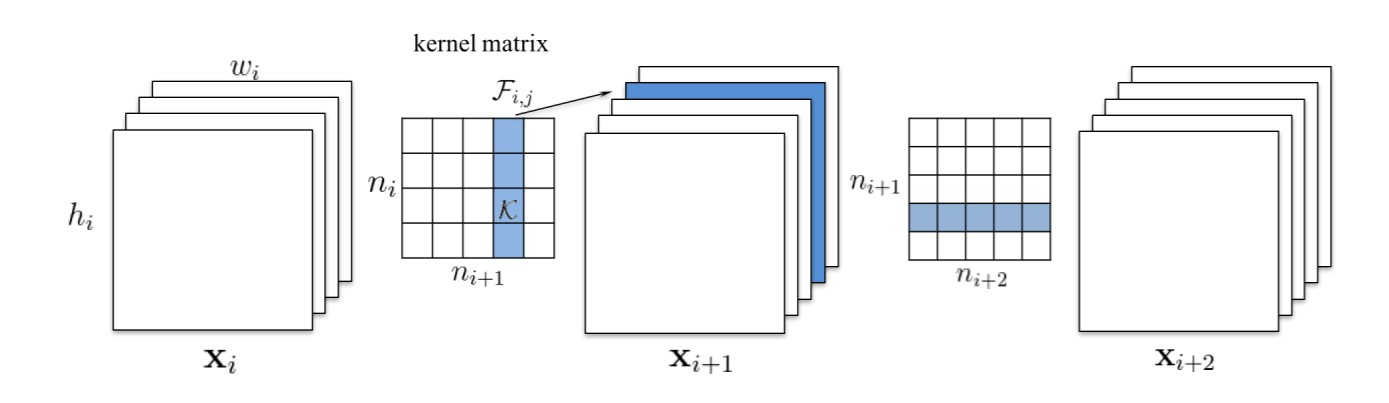
\includegraphics[width=\textwidth]{FilterPruning.jpg}
        \caption{Pruning a filter results in removal of its corresponding feature map and related kernels in the next layer.~\autocite{liPruningFiltersEfficient2017}}
        \label{fig:FeaturemapAndKernel}
    \end{figure}




%! ---------------------------------------------------------------------------------------------------------------------------------
\subsubsection{Model Selection}\label{sec:ModelSelection}

Pruning CNNs like AlexNet, or VGGNet is fairly straightforward, we can prune filters in any layer without worrying about damaging the fundamental structure of the network, however this is not the case with ResNets (short for Residual Networks),  a very popular type of CNN that makes use of what is known as a `residual block' (Figure~\ref{fig:ResidualBlock} shows a residual block) which, from the perspective of pruning, adds additional interdependencies between layers.

We selected ResNet56 as the target network because it is one of the few networks with prebuilt `off-the-shelf' schedules that also uses residual blocks. 
Performing this experiemnt on networks using residual blocks is important because the necessity of using compression techniques such as pruning increases as networks get larger, these residual blocks are very common in very large networks today. 

The pre-tuned pruning schedule publicly avaliable from Distiller has been hand built by an expert in the field, providing a solid baseline for comparison.
It is not a trivial task to improve on the pre-existing hand built schedules manually without extensive understanding of layer sensitivities.  

\begin{figure}[H]
    \centering
    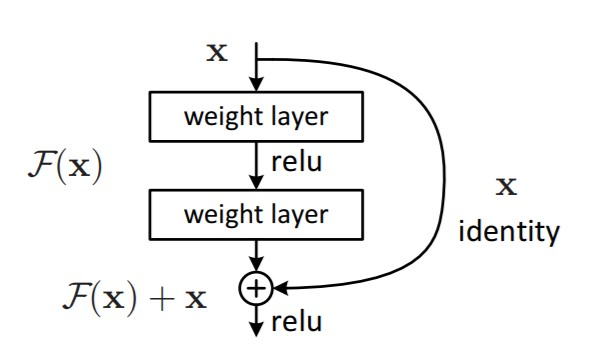
\includegraphics[width=0.5\textwidth]{ResidualBlock.jpg}
    \caption{A residual block, note the identity feature map skips the weight layers, this is also known as a `skip connection'.}
    \label{fig:ResidualBlock}
\end{figure}

\textbf{\color{red}Discuss further how residual blocks effect pruning.}
ResNets were originally proposed to help address a training accuracy degredation problem that can occur in very deep networks, Degredation (or accuracy saturation) occurs when adding more layers to a suitably deep model leads to higher training error~\autocite{heDeepResidualLearning2016}.
The accuracy degredation problem with very deep CNNs is common enough that many new deep networks in research and production make use of them today.

%! ---------------------------------------------------------------------------------------------------------------------------------
\subsubsection{Model Retraining}
\textbf{TBD}


\newpage
%! ---------------------------------------------------------------------------------------------------------------------------------
\subsection{Engineering/implementation details}
This section will discuss the specifics of the system engineered to perform the experiments.{\color{red}Rephase needed}
\subsubsection{High level overview of system}

Figure~\ref{fig:agentCommunication} shows how each system interacts in the pipeline, pruning is handled by the agent/s marked `Producer', benchmarking is handled by the `Consumer' agent, and the wandb system serves the next set of sweep parameters to each of the `Producer' agents.

\begin{figure}[H]
    \centering
    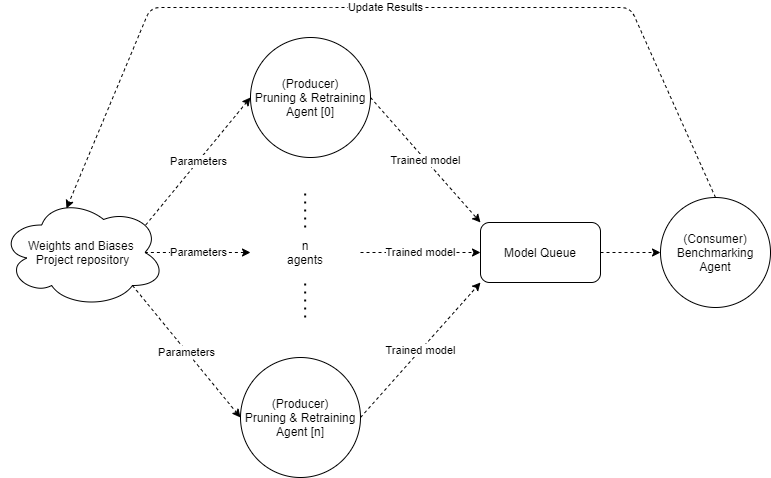
\includegraphics[width=\textwidth]{./ProducerConsumer}
    \caption{Diagram showing agent communication}
    \label{fig:agentCommunication}
\end{figure}

When pruning begins, the producer agent requests the (initially random) pruning parameters from the Weights and Biases Project server, the producer then applies the pruning algorithm and begins retraining the model.
Upon completion of retraining the model is exported into ONNX format and added to a queue for the consumer (the benchmarking agent) to benchmark and record the results, these results are then logged to weights and biases.
As described in Section~\textbf{(TBD)} the parameter importance and correlation with the target metric is re-computed each time results are logged this can help determine in what direction to tune the paramater settings to minimise (or maximise) the target metric.

The runtime of a full benchmark for one model on the NCS is usually at most 5 seconds, pruning and retraining the network however can take between 20 - 120 mins depending on the network size and number of epochs. 
To imporve the efficiency of the training we separated the benchmarking system (consumer) from the pruning and retraining systems (producer), this made it easy to add additional pruning and retraining agents to a single experiment or run multiple experiments in parallel.

%! ---------------------------------------------------------------------------------------------------------------------------------
\subsubsection{Defining parameters to prune}

\singlespacing
\begin{figure}[H]
    \begin{minted}[breaklines, linenos]{yaml}
        pruners: 
            layer_1_conv_pruner:
                class: 'L1RankedStructureParameterPruner'
                group_type: Filters
                desired_sparsity: 0.9
                weights: [
                    module.layer1.0.conv1.weight,
                    module.layer1.1.conv1.weight
                ]
        lr_schedulers:
            exp_finetuning_lr:
                class: ExponentialLR
            gamma: 0.95

        policies:
            - pruner:
                instance_name: layer_1_conv_pruner
                epochs: [0]
            
            - lr_scheduler:
                    instance_name: exp_finetuning_lr
                starting_epoch: 10
                ending_epoch: 300
                frequency: 1
    \end{minted}
    \caption{Example distiller schedule file, showing the pruning algorithm selected, and that algorithms parameters}
    \label{fig:CompressionSchedule}
\end{figure}
\doublespacing

Distiller uses a `compression schedule' file to define the behaviour of the compression algorithms used, Figure~\ref{fig:CompressionSchedule} shows a simple example compression schedule, with a definition for a single `pruner' instance (line 2 - \texttt{\color{mintedgreen}layer\_1\_conv\_pruner}), a single `\texttt{\color{mintedgreen}lr\_scheduler}' instance (line 11 - \texttt{\color{mintedgreen}exp\_fine\_tuning\_lr}), and their respecitve policies (explained below).


The pruning schedule is composed of lists of sections that describe `{\color{mintedgreen}pruners}', `{\color{mintedgreen}lr-schedulers}', and `{\color{mintedgreen}policies}'. 
A `{\color{mintedgreen}pruner}' defines a pruning algorithm and the layers on which that pruning algorithm will be applied, `LR-schedulers' define the \textbf{learning-rate decay(Definition required)} algorithm. 
Finally each policy references an instance of a pruner or LR-scheduler, and controls when the respective algorithm will be applied, such as the start and end epoch, and the frequency of application.

The example compression schedule shown in Figure~\ref{fig:CompressionSchedule} provides instructions to Distiller to use the `L1RankedStructureParameterPruner' algorithm (as described in Section~\ref{sec:FilterPruningAlgo}) to prune the weights in each of the convolutions described by the `weights' array, in this case `\texttt{\color{mintedgreen}group\_type}' specifies filter pruning and `\texttt{\color{mintedgreen}desired\_sparsity}' indicates how many tensors it will aim to remove (0.9 indicates the algorithm will attempt to remove 90\% of the tensors), desired sparsity should not be confused with an actual change in sparsity - note that filter and channel pruning will always result in a dense layer with an actual sparsity of 0 because this is a form of coarse-grained pruning (see section~\ref{sec:Pruning}).

\begin{figure}[H]
    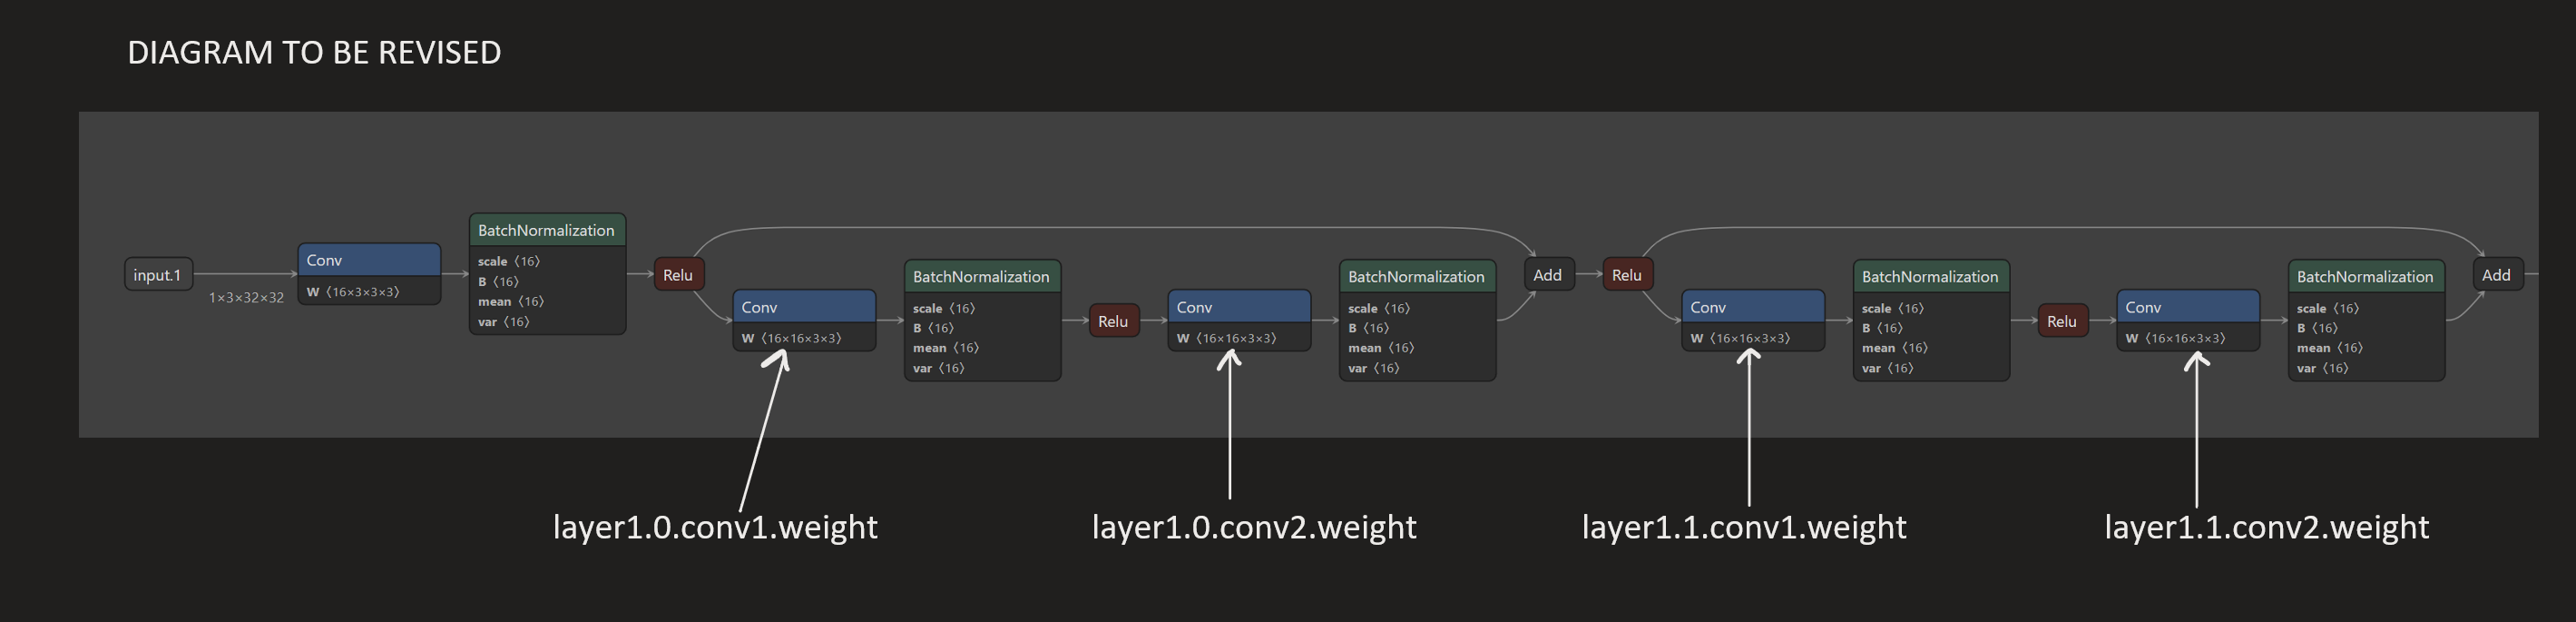
\includegraphics[width=\textwidth]{temp_pruning_layers.png}
    \caption{Resnet56 fragment showing first 2 residual block with the corresponding weights matrices labelled. \textbf{(TODO: rescale and redraw to highlight pertinent information)}}
    \label{fig:resnet56weightlabels}
\end{figure}

Each layer in the network is implicitly labelled (see figure~\ref{fig:resnet56weightlabels}), distiller uses these labels to identify which weight matricies are being referenced by the compression schedule. 


\newpage
%! ---------------------------------------------------------------------------------------------------------------------------------
\subsubsection{WandB API}

\singlespacing
\begin{figure}[H]
    \begin{minted}[breaklines]{yaml}
        program: pipeline.py
        method: bayes
        metric:
            goal: minimize
            name: Latency
        parameters:
            layer_1_conv_pruner_desired_sparsity:
                min: 0.01
                max: 0.99
            layer_1_conv_pruner_group_type:
                values: [Channels, Filters]
    \end{minted}
    \caption{WandB sweep configuration file}
    \label{fig:sweepConfig}
\end{figure}
\doublespacing

To explore the space of pruning paramater values the hyperparameter optimisation framework exposed by WandB called `Sweeps' was leveraged. 
This involves writing a python script that can run the entire pipeline (pruning, training \& benchmarking) and record the results, to accomplish this each sweep needs a configuration file (see Figure~\ref{fig:sweepConfig}), table~\ref{tab:WandBConfig} shows a desciption of each key in the wandb configuration file with a summary of appropriate arguments. 


% which needs a definition to the python script being run (program), the search strategy (method, either grid, random, or bayes), a metric  

\begin{table}[H]
    \begin{tabular}{@{}|l|l|l|@{}}
    \toprule
    Key        & Description                    & Value                                    \\ \midrule
    program    & Script to be run               & Path to script                           \\ \midrule
    method     & Search strategy                & grid, random, or bayse                   \\ \midrule
    metric     & The metric to optimise         & Name and direction of metric to optimise \\ \midrule
    parameters & The parameter bounds to search & Name and min/max or array of fixed values  \\ \bottomrule
    \end{tabular}
    \caption{Configuration setting keys, descriptions and values}
    \label{tab:WandBConfig}
\end{table}


%Each set of pruning parameters in this experiment used a bayesian optimisation technique~\autocite{snoekPracticalBayesianOptimization2012}


This configuration file tells wandb the names of the parameters to pass as arguments to the pipeline script with their expected value ranges, such as a list of strings or a min and max float/integer. 
The pipeline script that recieves the arguments from wandb contains a mapping from the wandb arguments to the corresponding value in the distiller compression schedule.
The pipeline then uses the values provided by wandb and writes out a new schedule that will be fed into distiller. 

%! ---------------------------------------------------------------------------------------------------------------------------------
\subsubsection{Benchmarking}

\begin{figure}[H]
	\centering
	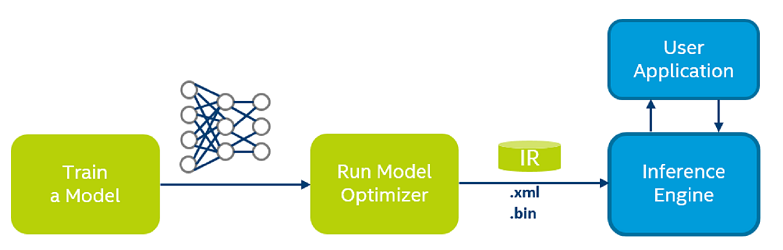
\includegraphics{./OpenVinoModelOptimizer}
	\caption{Workflow for deploying trained model onto NCS~\autocite{ModelOptimizerDeveloper}}
	\label{fig:OpenVinoWorkflow}
\end{figure}


To pass the pruned and trained model to the Neural Compute stick OpenVino was used, it is a toolkit providing a high level \textbf{inference engine(\color{red}Definition needed)} API, this facilitates the process of optimising the model for specialised hardware (in this case the NCS), and loading the optimised model into the hardware. 
OpenVino itself has a benchmarking tool that we leveraged to access detailed latency and throughput metrics; from end to end latency all the way down to the latency of each instruction used for inference on the VPU~\textbf{\color{red}link to example table of HW operations and latency in appendix}. 
Before starting the benchmark we convert the ONNX model into an Intermediate Representation (IR) format by running it through the model optimizer, the IR can then be read by the Inference Engine and loaded into VPU memory.
Once the model is loaded into VPU we load the images that will be used for benchmarking into the VPU memory.
We observe three measurements for every model, the end-to-end latency (from loading an image into the model until getting a result), the sum of latency for each instruction executed by the VPU once the image is loaded into memory, and finally we also measure the throughput (the number of images (frames) that can be processed per second or FPS).

%! ---------------------------------------------------------------------------------------------------------------------------------
\subsection{Experiment setup}
We conducted three experiments using the Resnet56 model trained on the CIFAR10 dataset. 
The first experiment set the retraining epochs to 0 so we could prune and benchmark rapidly, we set minimisation of latency to be the target.
For the second experiment we set the target to minimise latency, but this time allowed retraining up to 300 epochs.
The final (third) experiment was the same as the second but we set the target metric to maximise Top1 accuracy. 

\singlespacing
\noindent\textbf{Observed metrics:}
\begin{itemize}
    \item \textbf{Latency} | Computed by calculating the sum of CPU time for hardware operations inside the NCS after the model and images have been loaded into memory.
    \item \textbf{Total\_Latency} | Measures the full latency to perform inference on an image once a model is optimised and loaded into the NCS, inlcuding loading the image into the stick memory.
    \item \textbf{Throughput} | Shows the number of images per second that can be processed by the NCS.
    \item \textbf{Top1} | The \% accuracy of the most likely class the model predicts.
    \item \textbf{Top5} | The \% accuracy of the top 5 predicted classes.
\end{itemize}
\doublespacing

\newpage
\subsubsection{Schedules}
Table~\ref{tab:scheduleWeights} shows how the weights are grouped and labeled for Filter pruning in the selected Resnet56 model, the 3 labelled pruners and their corresponding weights were used in all experiments.
Layers with a similar degree of sensitivity to pruning are grouped together, layers that are omitted from the table have a much higher sensitivity to pruning and are not pruned at all, pruning more sensitive layers can result in a significantly higher rate of pruned neural networks that lose all predictive ability.
Grouping layers in this way helps us avoid having to use 56 pruning parameters (one for each layer per residual block) and significantly reduces the complexity of the parameter search.\\

Note that only the first convolution in each residual block is being pruned, because the convolutions following this will also have the kernels removed following the removed feature maps (See Section~\ref{sec:ModelSelection}).

\singlespacing
\begin{table}[H]
    \centering
    \setlist[itemize]{font= \color{black}, wide, leftmargin=*, noitemsep, after=\vspace*{-\topsep}}
    \setlength{\extrarowheight}{0.5pt}
    \setlength{\tabcolsep}{3pt}
    \begin{tabularx}{0.6\textwidth}{|p{40mm}|*{1}{>{\compress\RaggedRight\arraybackslash} X |}}
    \hline
    Label & Weights  \\
    \hline
    filter\_pruner\_layer\_1
    & \begin{itemize}
        \item module.layer1.0.conv1.weight
        \item module.layer1.1.conv1.weight
        \item module.layer1.2.conv1.weight
        \item module.layer1.3.conv1.weight
        \item module.layer1.4.conv1.weight
        \item module.layer1.5.conv1.weight
        \item module.layer1.6.conv1.weight
        \item module.layer1.7.conv1.weight
        \item module.layer1.8.conv1.weight
    \end{itemize} \\ 
    \hline
    filter\_pruner\_layer\_2 
    & \begin{itemize}
        \item module.layer2.1.conv1.weight
        \item module.layer2.2.conv1.weight
        \item module.layer2.3.conv1.weight
        \item module.layer2.4.conv1.weight
        \item module.layer2.6.conv1.weight
        \item module.layer2.7.conv1.weight
    \end{itemize} \\ 
    \hline
    filter\_pruner\_layer\_3.1
    & \begin{itemize}
        \item module.layer3.1.conv1.weight
    \end{itemize} \\
    \hline
    filter\_pruner\_layer\_3.2
    & \begin{itemize}
        \item module.layer3.2.conv1.weight
        \item module.layer3.3.conv1.weight
        \item module.layer3.5.conv1.weight
        \item module.layer3.6.conv1.weight
        \item module.layer3.7.conv1.weight
        \item module.layer3.8.conv1.weight
    \end{itemize}\\ \hline
    \end{tabularx}
    \caption{Mapping of pruners to filter weights}
    \label{tab:scheduleWeights}
\end{table}
\doublespacing

\subsubsection{Passing pruned/trained networks to benchmarker}
\emph{Discuss reading/writing yaml files, outputting .onnx files, redis to pass messages between agents}

\subsubsection{Baseline data}
For the purposes of all experiments we compare our results to two baseline sets of data, first the basic ResNets56 network with pretrained weights for CIFAR10, and second an `off-the-shelf' version of ResNet56 with parameters hand picked by an expert in the field (\textbf{\color{red}qualify this?})~\autocite{liPruningFiltersEfficient2017}.

\subsubsection{Experiment 1: Rapid pruning, no retraining}


\subsubsection{Experiment 2: Target latency, with retraining}
This experiment targeted pure inference latency, no information regarding accuracy was encoded in the optimisation metric. 

\subsubsection{Experiment 3: Target Top1, with retraining}

\end{document}